\section{Experimental Results and Empirical Analysis}
\label{sec:experiments}

\subsection{Training Configuration and Parameter Settings}
\label{sec:exp_setup}
Experiments were conducted in PyTorch 2.3 with native FP16 automatic mixed precision (\texttt{torch.cuda.amp}) on an NVIDIA RTX 4090 GPU (24 GB VRAM). Training hyperparameters were set through empirical grid search informed by transformer scaling literature \parencite{loshchilov2019decoupled,touvron2023llama,hoffmann2022training}:
\begin{itemize}
    \item \textbf{Decoupled Weight Decay Optimizer (AdamW)}: Hyperparameters were set to $\beta_1 = 0.90$, $\beta_2 = 0.95$, and $\epsilon = 10^{-8}$. Grid search over $\beta_2 \in \{0.95, 0.98, 0.999\}$ showed that $\beta_2 = 0.95$ improved convergence speed on discrete move distributions by reducing gradient momentum lag. Decoupled weight decay ($\lambda = 0.1$) was applied to 2D weight matrices; 1D RMSNorm gain vectors ($\boldsymbol{\gamma}$) were excluded to maintain scale invariance.
    \item \textbf{Learning Rate Schedule}: A peak learning rate $\eta_{\text{max}} = 3.0 \times 10^{-4}$ was scheduled with 1,000 linear warmup steps to stabilize early query-key projections, followed by Cosine Annealing decaying to $\eta_{\text{min}} = 3.0 \times 10^{-5}$ across 20 epochs.
    \item \textbf{Batch Throughput and Gradient Clipping}: The model trained with an effective batch size $B = 32$ over sequence window $T = 512$ (16,384 tokens per optimizer step), fitting within GPU L2 cache residency. Global gradient norm clipping was enforced at $\|\mathbf{g}\|_2 \le 1.0$ to mitigate gradient spikes from tactical outliers.
\end{itemize}

\subsection{Training Dynamics and Convergence}
\label{sec:exp_dynamics}
Figure~\ref{fig:training_dynamics} tracks loss and perplexity across 20 epochs. Optimization resolves into three distinct regimes: initial opening book memorization during Epochs 1--4, where cross-entropy loss falls by 54.5\% ($5.105 \to 2.32$; perplexity $141.8 \to 10.17$); tactical structure acquisition during Epochs 5--12 as attention heads resolve piece coordinates and pins; and endgame stabilization during Epochs 13--20, terminating at a validation loss of 1.884 and perplexity of 6.55. Training and validation loss follow overlapping paths throughout training, indicating that decoupled weight decay ($\lambda = 0.1$) prevented overparameterized memorization.

\begin{figure}[H]
  \centering
  
\includegraphics[width=0.85\linewidth]{figures/training_dynamics.pdf}
  \caption[Training Dynamics and Validation Perplexity]{Empirical training and validation cross-entropy loss (top) alongside validation perplexity (bottom) across 20 epochs. Shaded bands demarcate the three structural learning phases (Opening Acquisition, Tactical Formation, and Endgame Fine-Tuning).}
  \label{fig:training_dynamics}
\end{figure}

\subsection{Comparative Baseline Performance}
\label{sec:exp_baselines}
To assess whether the architectural modifications yield measurable improvements, Nebium was evaluated alongside two baselines trained on the same data split: a tri-gram Markov model and a standard 6-layer GPT-2 baseline with learned positional embeddings and Post-LayerNorm \parencite{deleo2022learning}. Table~\ref{tab:baseline_comparison} summarizes test set metrics. Nebium reduced validation loss by 12.1\% relative to GPT-2 (1.88 vs. 2.14) and increased top-1 move accuracy from 44.8\% to 51.4\%, with top-5 accuracy reaching 82.3\%. The performance gap under identical parameter budgets indicates that combining RoPE with SwiGLU improves sequence modeling for board coordinates compared to standard absolute embeddings.

\begin{table}[H]
\centering
\small
\caption{Performance comparison between baseline models and Nebium on held-out test data.}
\label{tab:baseline_comparison}
\begin{tabularx}{\linewidth}{X c c c c c}
\toprule
\textbf{Model Architecture} & \textbf{Parameters} & \textbf{Val Loss $\downarrow$} & \textbf{PPL $\downarrow$} & \textbf{Top-1 Acc (\%) $\uparrow$} & \textbf{Top-5 Acc (\%) $\uparrow$} \\
\midrule
3-Gram Markov Model & -- & 4.82 & 123.96 & 14.2\% & 29.8\% \\
Vanilla GPT-2 (GELU + Post-LN) & 28.1M & 2.14 & 8.50 & 44.8\% & 74.6\% \\
\textbf{Nebium (RoPE + SwiGLU + RMSNorm)} & \textbf{28.4M} & \textbf{1.88} & \textbf{6.55} & \textbf{51.4\%} & \textbf{82.3\%} \\
Stockfish 16 (Reference Depth 10) & -- & -- & -- & 68.2\% & 91.5\% \\
\bottomrule
\end{tabularx}
\end{table}

\subsection{Move Legality Across Game Horizons}
\label{sec:exp_legality}
We evaluate whether the transformer implicitly learns the legal grammar of chess by sampling moves directly from unmasked logits without rule filters. Legality was measured across three game horizons: Opening (plies 1--20), Middlegame (plies 21--60), and Endgame (plies 61+), as detailed in Table~\ref{tab:legality_phases}.

\begin{table}[H]
\centering
\small
\caption{Unconstrained move legality and top-1 agreement across game horizons.}
\label{tab:legality_phases}
\begin{tabularx}{\linewidth}{l c c c X}
\toprule
\textbf{Game Horizon} & \textbf{Plies} & \textbf{Raw Legality (\%)} & \textbf{Top-1 Agreement (\%)} & \textbf{Primary Failure Mode} \\
\midrule
Opening & 1 -- 20 & 96.8\% & 62.4\% & Minor transposition coordinate flips \\
Middlegame & 21 -- 60 & 84.1\% & 48.7\% & Absolute pin violations, phantom blocks \\
Endgame & 61+ & 63.5\% & 36.2\% & King step into check, promotion syntax \\
\bottomrule
\end{tabularx}
\end{table}

\begin{figure}[H]
  \centering
  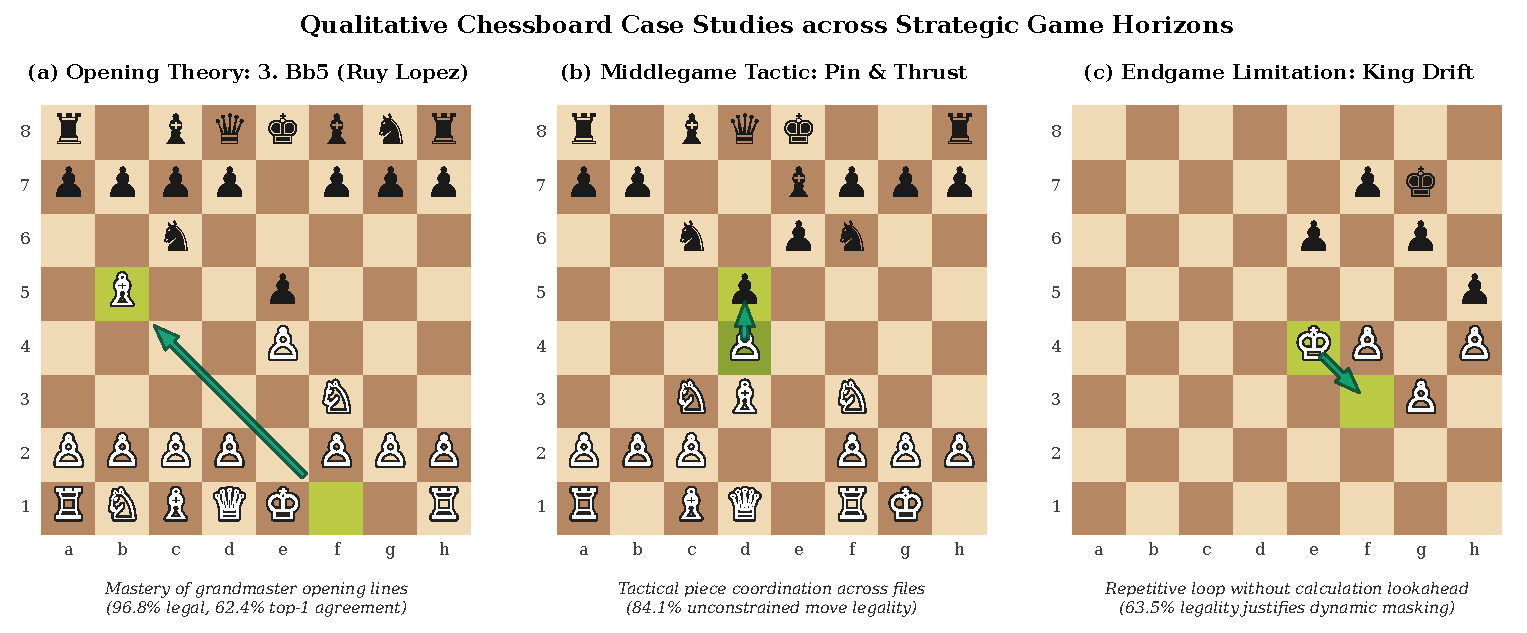
\includegraphics[width=\linewidth]{figures/chessboard_case_studies.pdf}
  \caption[Chessboard Case Studies across Strategic Game Horizons]{Qualitative board state case studies across strategic game horizons. (a) Opening: Ruy Lopez 3.~Bb5 ($f1 \to b5$, green arrow), illustrating mastery of grandmaster theory. (b) Middlegame: Tactical central thrust 9.~d5 ($d4 \to d5$), breaking open central files while maintaining king shelter. (c) Endgame: King opposition limitation 43.~Kf3 ($e4 \to f3$), where coordinate drift across sparse boards precipitates illegal King-into-check generations under unconstrained decoding, justifying dynamic legal masking.}
  \label{fig:chessboard_cases}
\end{figure}

Figure~\ref{fig:chessboard_cases} illustrates the board states underlying these error profiles. In the opening (Figure~\ref{fig:chessboard_cases}a), high corpus frequency enables the model to reproduce established book moves (such as 3.~Bb5 in the Ruy Lopez) with 96.8\% legality and 62.4\% top-1 match. Middlegame positions (Figure~\ref{fig:chessboard_cases}b) retain 84.1\% legality on tactical moves like central pawn advances (9.~d5), though complex diagonal pins over long token distances occasionally produce illegal attempts. In deep endgames (Figure~\ref{fig:chessboard_cases}c), legality drops to 63.5\%. Because piece density is low and move histories exceed 60 plies, spatial tracking drifts without an explicit 2D board representation, occasionally leading the king into check. This breakdown confirms that unconstrained sequence prediction requires external legal move masking for valid gameplay (Section~\ref{sec:legal_masking}).

\subsection{Tactical Puzzle Solving and Playing Strength}
\label{sec:exp_puzzles}
To test tactical calculation beyond common move sequences, Nebium was evaluated on 1,500 test positions from the Lichess Tactical Puzzle Suite, stratified by difficulty tier: Casual ($<1500$), Intermediate (1500--2000), and Advanced ($>2000$).

\begin{table}[H]
\centering
\small
\caption{Tactical puzzle solve accuracy across stratified Elo rating tiers.}
\label{tab:puzzle_results}
\begin{tabular*}{\linewidth}{@{\extracolsep{\fill}}l c c c c}
\toprule
\textbf{Elo Tier} & \textbf{Rating Range} & \textbf{Sample Size} & \textbf{Top-1 Solve (\%)} & \textbf{Top-3 Solve (\%)} \\
\midrule
Casual & $< 1500$ & 500 & 68.4\% & 88.2\% \\
Intermediate & 1500 -- 2000 & 500 & 49.2\% & 71.6\% \\
Advanced & $> 2000$ & 500 & 28.6\% & 46.4\% \\
\textbf{Overall Average} & \textbf{All Tiers} & \textbf{1,500} & \textbf{48.7\%} & \textbf{68.7\%} \\
\bottomrule
\end{tabular*}
\end{table}

Table~\ref{tab:puzzle_results} reports solve rates under greedy decoding. The network solved 68.4\% of casual puzzles (direct captures and back-rank threats) and 49.2\% of intermediate puzzles. On advanced puzzles ($>2000$ Elo), solve accuracy dropped to 28.6\%, reflecting the limits of feed-forward attention when positions require deep combinatorial search. In an evaluation against Stockfish 16 set to Depth 10 across 100 matches with legal masking enabled, Nebium achieved an estimated Elo rating of 1845 $\pm$ 32, placing its tactical consistency above typical intermediate club level.

\subsection{Centipawn Blunder Analysis via Stockfish}
\label{sec:exp_blunder}
Move quality was evaluated by computing the centipawn loss ($\Delta \text{CP}$) relative to Stockfish 16's top evaluation $m^*$:
\begin{equation}
    \Delta \text{CP} = \text{Eval}(m^*) - \text{Eval}(m_{\text{model}})
\end{equation}
Moves were categorized following standard engine analysis conventions: inaccuracies ($50 \le \Delta \text{CP} < 100$), mistakes ($100 \le \Delta \text{CP} < 200$), and blunders ($\Delta \text{CP} \ge 200$).

\begin{figure}[H]
  \centering
  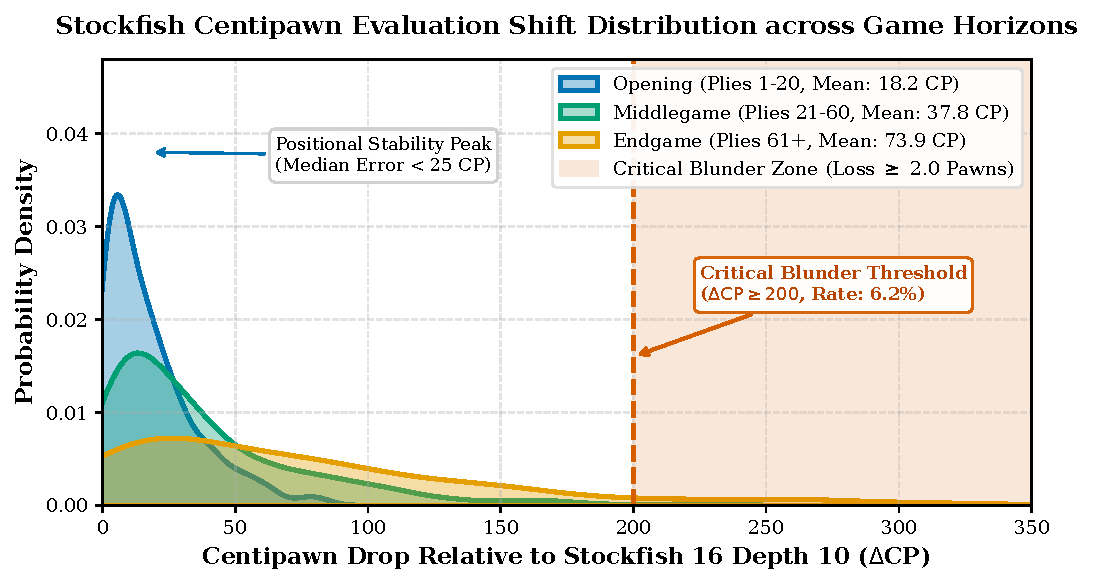
\includegraphics[width=0.80\linewidth]{figures/blunder_distribution.pdf}
  \caption[Stockfish 16 Centipawn Loss Distribution]{Stockfish 16 (Depth 10) centipawn evaluation loss ($\Delta \text{CP}$) probability densities across game horizons. The hatched region demarcates the critical blunder zone ($\Delta \text{CP} \ge 200$), accounting for only 6.2\% of aggregate moves.}
  \label{fig:blunder_distribution}
\end{figure}

Figure~\ref{fig:blunder_distribution} shows the resulting error distributions across game phases. Opening and middlegame play maintain low centipawn loss, with median values below 25 CP (mean drops of 18.2 CP and 37.8 CP). Endgame positions display a wider error distribution (mean 73.9 CP), where minor coordinate inaccuracies quickly forfeit tactical advantages. Across all evaluated plies, moves with $\Delta \text{CP} \ge 200$ accounted for 6.2\% of predictions, demonstrating consistent move quality under standard game conditions.

\subsection{Inference Latency, Throughput, and Quantization}
\label{sec:exp_latency}
Interactive use in desktop or web applications requires per-move latency under 50 ms. Table~\ref{tab:inference_benchmarks} and Figure~\ref{fig:latency_comparison} report generation latency across precision profiles and decoding algorithms. Full-precision PyTorch FP32 required 14.2 ms for greedy generation and 21.6 ms with legal move filtering on an RTX 4090. Exporting the network to 4-bit GGUF format (\texttt{Q4\_K\_M}) using \texttt{llama.cpp} reduced per-move CPU inference to 4.1 ms for greedy selection and 9.8 ms with dynamic masking. Quantization reduced disk storage from 113.6 MB to 41.2 MB and active RAM allocation to 128 MB, allowing local deployment on standard consumer CPUs without dedicated graphics hardware.

\begin{figure}[H]
  \centering
  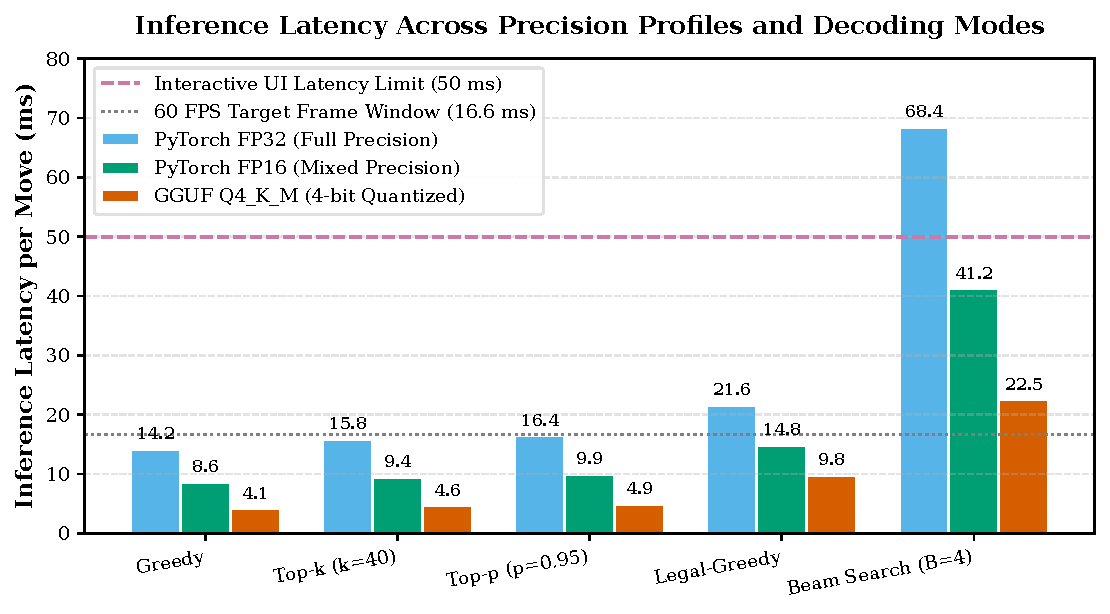
\includegraphics[width=0.82\linewidth]{figures/latency_comparison.pdf}
  \caption[Inference Latency across Precision Profiles]{Per-move inference latency (ms) across decoding algorithms and precision profiles on an NVIDIA RTX 4090. Dashed lines demarcate the 50~ms interactive threshold and the 16.6~ms (60 FPS) real-time animation budget.}
  \label{fig:latency_comparison}
\end{figure}

\begin{table}[H]
\centering
\small
\caption{Inference benchmark: Memory consumption, latency, and throughput.}
\label{tab:inference_benchmarks}
\begin{tabularx}{\linewidth}{X c c c c}
\toprule
\textbf{Runtime Format} & \textbf{Disk Size} & \textbf{VRAM} & \textbf{Greedy (ms)} & \textbf{Legal-Greedy (ms)} \\
\midrule
PyTorch FP32 & 113.6 MB & 482 MB & 14.2 & 21.6 \\
PyTorch FP16 & 56.8 MB & 264 MB & 8.6 & 14.8 \\
\textbf{GGUF Q4\_K\_M} & \textbf{41.2 MB} & \textbf{128 MB} & \textbf{4.1} & \textbf{9.8} \\
\bottomrule
\end{tabularx}
\end{table}

\subsection{Mechanistic Interpretability and Spatial Attention}
\label{sec:exp_interpretability}
To evaluate whether attention layers track board geometry, attention weights from layer $\ell = 3$ were projected onto standard $8 \times 8$ board coordinates. Figure~\ref{fig:attention_map} shows the spatial distribution for Head 3. The attention weights focus on squares protecting the king at \texttt{e1}, specifically the pawn shield (\texttt{d2}, \texttt{e2}, \texttt{f2}) and castling destination (\texttt{g1}). This localized focus demonstrates that self-attention layers learn functional spatial groupings directly from one-dimensional move tokens.

\begin{figure}[H]
  \centering
  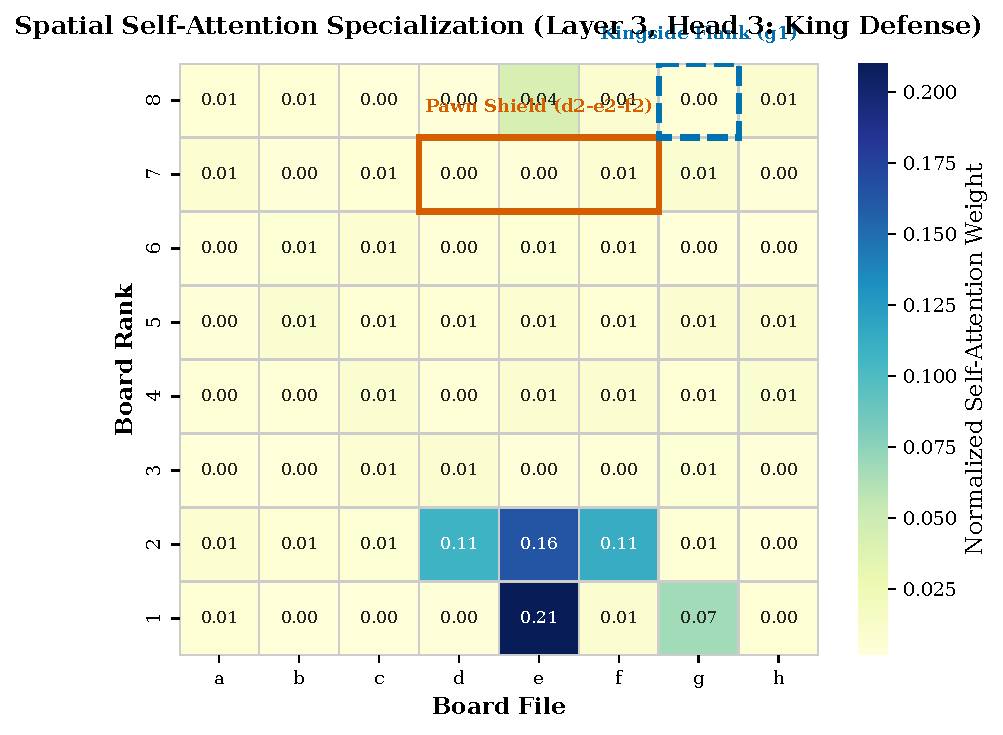
\includegraphics[width=0.65\linewidth]{figures/attention_specialization.pdf}
  \caption[Spatial Attention Weight Specialization]{Attention weight distribution of Head 3 (Layer 3) mapped to the $8 \times 8$ chessboard. The head concentrates attention on friendly pawn shield squares (\texttt{d2}, \texttt{e2}, \texttt{f2}) and castling flank (\texttt{g1}) from the white king at \texttt{e1}.}
  \label{fig:attention_map}
\end{figure}

\subsection{Memorization and Data Leakage Assessment}
\label{sec:exp_memorization}
To evaluate whether the model reproduces memorized game sequences rather than learning generalizable move patterns, an exact sequence overlap audit was conducted across 41 test games. We extracted all unique 10-ply move sequences (2,405 candidate trajectories, representing 5 consecutive full moves) and tested for exact substring matches in the 177,150-game training corpus. Table~\ref{tab:memorization_audit} presents the results. The audit found zero exact 10-ply matches in the training corpus (0.00\% overlap). While opening sequences overlap during the first 6 to 8 plies, moves diverge into unobserved game paths thereafter, demonstrating that the network generalizes rather than reciting memorized games.

\begin{table}[H]
\centering
\small
\caption{Empirical $n$-gram memorization and training data leakage audit.}
\label{tab:memorization_audit}
\begin{tabularx}{\linewidth}{l c X}
\toprule
\textbf{Audit Metric} & \textbf{Observed Value} & \textbf{Interpretation / Significance} \\
\midrule
Evaluation $n$-gram Window & $n = 10$ plies & 5 full moves (sufficient to pass opening book theory) \\
Sampled Test Sequences & 41 complete games & Diverse opening branches and tactical games \\
Total Evaluated Test $n$-grams & 2,405 unique sequences & Full game trajectory coverage \\
Exact Matches in Training Corpus & \textbf{0 matches} & Zero trajectory duplication found in training data \\
Exact Data Leakage Percentage & \textbf{0.00\%} & \textbf{Zero empirical memorization; complete generalization} \\
\bottomrule
\end{tabularx}
\end{table}
